\documentclass[tikz,border=12pt]{standalone}
% Estilo comum dos esquemas vetoriais das aulas da GA033.
\usepackage[T1]{fontenc}
\usepackage[utf8]{inputenc}
\usepackage{lmodern}
\usepackage{amsmath,amssymb}
\usetikzlibrary{arrows.meta,positioning,calc,fit,matrix,decorations.pathreplacing,backgrounds,shapes.geometric}
\definecolor{lnccblue}{HTML}{075AC0}
\definecolor{ink}{HTML}{242A31}
\definecolor{muted}{HTML}{647080}
\definecolor{lightblue}{HTML}{EFF5FC}
\definecolor{teal}{HTML}{197C83}
\definecolor{orange}{HTML}{BC6A16}
\tikzset{
  every node/.style={font=\sffamily\fontsize{15}{18}\selectfont,text=ink},
  box/.style={draw=lnccblue,line width=0.9pt,fill=lightblue,inner sep=9pt,align=center},
  flow/.style={-{Stealth[length=3mm,width=2mm]},draw=lnccblue,line width=1pt},
  point/.style={circle,draw=lnccblue,fill=white,line width=1.2pt,minimum size=3.2mm,inner sep=0pt},
  label/.style={font=\sffamily\fontsize{13}{16}\selectfont,text=muted},
  heading/.style={font=\sffamily\bfseries\fontsize{16}{19}\selectfont,text=lnccblue}
}
% Impede setas horizontais involuntariamente invertidas após editar os nós.
\newdimen\origemseta
\newdimen\destinoseta
\newcommand{\verificarsetadireita}[2]{%
  \pgfextractx{\origemseta}{\pgfpointanchor{#1}{east}}%
  \pgfextractx{\destinoseta}{\pgfpointanchor{#2}{west}}%
  \advance\origemseta by 4mm%
  \ifdim\destinoseta>\origemseta\else
    \PackageError{diagramas}{Conector sem espaco entre #1 e #2}{Afaste os nos antes de compilar.}%
  \fi
}

\begin{document}
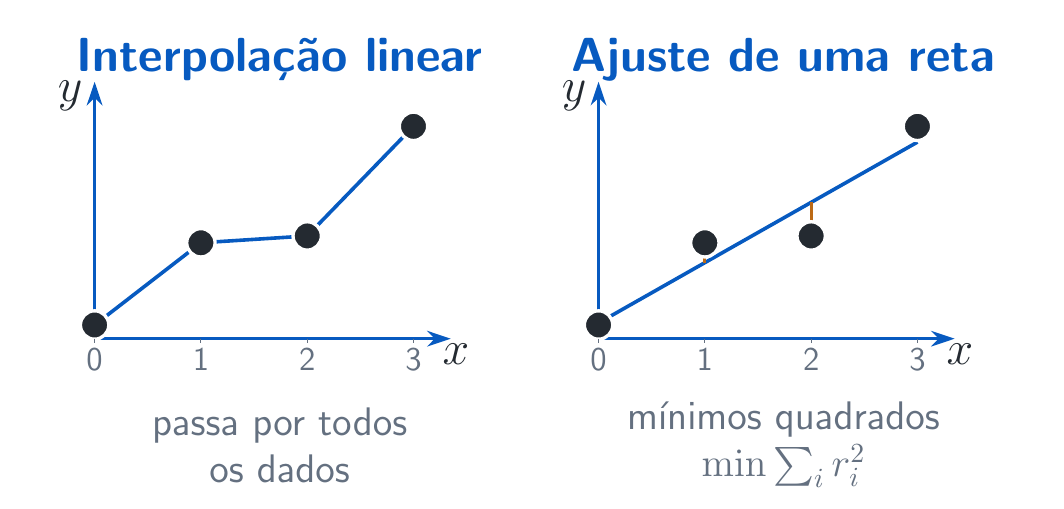
\begin{tikzpicture}[x=1cm,y=1cm,
  every node/.append style={font=\sffamily\fontsize{16}{19}\selectfont}]
  \path[use as bounding box] (0,-.85) rectangle (12.8,4.9);
  \node[heading] at (3.2,4.5) {Interpolação linear};
  \node[heading] at (9.6,4.5) {Ajuste de uma reta};
  \begin{scope}[shift={(.85,.95)},x=1.35cm,y=.87cm]
    \draw[flow] (0,0) -- (3.35,0);
    \draw[flow] (0,0) -- (0,3.75);
    \node at (3.4,-.22) {$x$};
    \node at (-.23,3.55) {$y$};
    \draw[lnccblue,line width=1.3pt] plot coordinates {(0,.2) (1,1.4) (2,1.5) (3,3.1)};
    \foreach \xx/\yy in {0/.2,1/1.4,2/1.5,3/3.1} {
      \node[point,fill=ink,draw=white,minimum size=3.6mm] at (\xx,\yy) {};
    }
    \foreach \xx in {0,1,2,3} {
      \draw[muted] (\xx,0) -- (\xx,-.07);
      \node[text=muted,font=\sffamily\fontsize{13}{16}\selectfont] at (\xx,-.3) {\xx};
    }
  \end{scope}
  \begin{scope}[shift={(7.25,.95)},x=1.35cm,y=.87cm]
    \draw[flow] (0,0) -- (3.35,0);
    \draw[flow] (0,0) -- (0,3.75);
    \node at (3.4,-.22) {$x$};
    \node at (-.23,3.55) {$y$};
    \draw[lnccblue,line width=1.3pt] (0,.23) -- (3,2.87);
    \foreach \xx/\yy in {0/.2,1/1.4,2/1.5,3/3.1} {
      \draw[orange,line width=1.1pt] (\xx,\yy) -- (\xx,{.88*\xx+.23});
      \node[point,fill=ink,draw=white,minimum size=3.6mm] at (\xx,\yy) {};
    }
    \foreach \xx in {0,1,2,3} {
      \draw[muted] (\xx,0) -- (\xx,-.07);
      \node[text=muted,font=\sffamily\fontsize{13}{16}\selectfont] at (\xx,-.3) {\xx};
    }
  \end{scope}
  \node[text=muted,align=center,text width=5.4cm,font=\sffamily\fontsize{14}{17}\selectfont] at (3.2,-.4) {passa por todos\\os dados};
  \node[text=muted,align=center,text width=5.4cm,font=\sffamily\fontsize{14}{17}\selectfont] at (9.6,-.4) {mínimos quadrados\\$\min\sum_i r_i^2$};
\end{tikzpicture}
\end{document}
